 \title{Mid-term exam in FYS4170, Autumn 2012}
\author{
        Candidate number 11 \\
                University of Oslo\\
}

\documentclass[12pt]{article}
\usepackage{amsmath}
\usepackage{fullpage}
\usepackage{amsthm}
\usepackage{amsfonts}
\usepackage{graphicx}
\usepackage[english, norsk]{babel}
\usepackage[T1]{fontenc}
\usepackage{subfigure}
\usepackage{epstopdf}
\usepackage[hyphens]{url}
\usepackage{gensymb}
\usepackage{verbatim}
\usepackage{slashed}
\usepackage{amssymb}

\newtheorem{thm}{Theorem}

%% Define a new 'leo' style for the package that will use a smaller font.
\makeatletter
\def\url@leostyle{%
  \@ifundefined{selectfont}{\def\UrlFont{\sf}}{\def\UrlFont{\small\ttfamily}}}
\makeatother
%% Now actually use the newly defined style.
\urlstyle{leo}


%\usepackage[utf8]{inputenc}
%\usepackage{textcomp}
%\usepackage[T1]{fontenc}




\newcommand{\Fig}[1]{Figure~\ref{#1}}
\newcommand{\fig}[1]{figure~\ref{#1}}
\newcommand{\eq}[1]{equation~\ref{#1}}
\newcommand{\Eq}[1]{Equation~\ref{#1}}

% Shortcuts for including equations
\newcommand{\beq}{\begin{equation}}
\newcommand{\eeq}{\end{equation}}
\def\i{\hat{i}}
\def\j{\hat{j}}
\def\k{\hat{k}}
\def\uvec{\textbf{u}}
\def\vvec{\textbf{v}}
\def\xvec{\textbf{x}}


% Document formatting
\setlength{\parindent}{0mm}
\setlength{\parskip}{1.5mm}

% Hyper refs
\usepackage[pdftex,colorlinks,breaklinks]{hyperref}
\usepackage{listings}
\usepackage{color}
\usepackage{textcomp}
\definecolor{listinggray}{gray}{0.9}
\definecolor{lbcolor}{rgb}{0.9,0.9,0.9}
\definecolor{pink}{RGB}{255, 119, 255}
\lstset{
	backgroundcolor=\color{lbcolor},
	tabsize=4,
	rulecolor=,
	language=c++,
        basicstyle=\scriptsize,
        upquote=true,
        aboveskip={1.5\baselineskip},
        columns=fixed,
        showstringspaces=false,
        extendedchars=true,
        breaklines=true,
        prebreak = \raisebox{0ex}[0ex][0ex]{\ensuremath{\hookleftarrow}},
        frame=single,
        showtabs=false,
        showspaces=false,
        showstringspaces=false,
        identifierstyle=\ttfamily,
        keywordstyle=\color[rgb]{0,0,1},
        commentstyle=\color[rgb]{0.133,0.545,0.133},
        stringstyle=\color[rgb]{0.627,0.126,0.941},
	title=\lstname
}

\newcounter{subproject}
\renewcommand{\thesubproject}{\alph{subproject}}
\newenvironment{subproj}{
\begin{description}
\item[\refstepcounter{subproject}(\thesubproject)]
}{\end{description}}
\date{\today}

\begin{document}
 \section*{Verification of the method}
 In order to make sure the solver is free of bugs, we need to run it through some test solutions. Natural choices that should be reproduced exactly is the constant solution (for instance, $u(x,y,t) = 1.2$) and a plug wave. For python based programs, these tests can be put into a nosetest module, and done in \verb nose_test_betterwave.py  which can be found in the project folder. We there let each test run over all versions of the code (scalar, vectorized and (ideally) c++). For a constant solution we may create an initial state by
 \begin{lstlisting}[language=Python]
def I(x, y):
	return 1.2
 \end{lstlisting}
and test the output of the solver, $u$, through for instance:
\begin{lstlisting}[language=Python]
u_exact = 1.2*np.ones((Nx+1,Ny+1))
diff = np.abs(u_exact - u).max()
nt.assert_almost_equal(diff, 0, delta=1E-14)
\end{lstlisting}

 For the plug wave, we can do a very similar test, as long as we make sure the wave travels for exactly, and integer number of periods, so that the wave in the exact same state as it was initially. In the nosetest module this was done by trial and error while using a relatively coarse grid. We made the initial state by the function
  \begin{lstlisting}[language=Python]
def I(x, y):
		return np.logical_and((np.abs(x) < Lx/2.+1), (np.abs(x) > Lx/2.-1))*1.
 \end{lstlisting}
and test the output of the solver, $u$, through for instance:
\begin{lstlisting}[language=Python]
x = np.linspace(0, Lx, Nx+1)  # mesh points in x dir
y = np.linspace(0, Ly, Ny+1)  # mesh points in y dir
X,Y = np.meshgrid(x,y)
u_exact = I(X,Y)
T = 1.0
n = int(T/dt - 5)
fname = 'solution_%06d.txt' % n
u = np.loadtxt(fname)
diff = np.abs(u_exact - u[:,0]).max()
nt.assert_almost_equal(diff, 0, delta=1E-14)
\end{lstlisting}
 where the suitable value for $n$ had to be found manually.

Once these tests are passed, we began looking at the convergence rate of the solvers. In order to do this, we note in theory, the error in the solution should to lowest order behave as 
\begin{equation}\label{eq:errororder}
 E = C_1 (\Delta x)^2 + C_2(\Delta y)^2 + C_3(\Delta t)^2
\end{equation}
So that if we double the amount of mesh points in both time and space, we should reduce the error by a factor of 4. In order to measure the error, we decided to run the solver up to a given time (for simplicity, $T = 1.0$), and compare the solution to the exact solution some manufactured function in each point $(x_i,y_j)$. If we denote this error by $e_{i,j}$, then a reasonable expression for the total error would be 
\begin{equation}\label{eq:errorestimate}
 E = \left( \frac{1}{NxNy}\sum_{i,j} e_{i,j}^2 \right)^{1/2}.
\end{equation}
And so we check if this error is reduced by roughly a factor 4 if we double the number of grid points. Since this is only an estimate of the error behavior we will need to be a bit gentle on this requirement, and so we should check that the ratio between consecutive errors is, for instance, 1/4 up to an accuracy of $\pm 0.05$. We decided to test this on the standing wave solution 
\begin{equation}
 u(x,y,t) = e^{-bt}\cos\left(\frac{m_x \pi x }{L_x}\right)\cos\left(\frac{m_y \pi y }{L_y}\right)\cos(\omega t)
\end{equation}
with source and initial state as described in section (TODO:find the right section after merge). A test for convergence rate may look something like
\begin{lstlisting}[language=Python]
mx = 4.; my = 4.; b = 0.01; omega=np.pi;
def u_exact(x,y,t):
	return ...
def f(x,y,t):
	return ...
def I(x, y):
	return ...
def V(x,y):
	return ...
Nx = 40; Ny = 40; T = 1.0
dt = 0.01
for version in ['vectorized']:
	errorlist=[0,0,0]
	for i in range(3):	
		... # construct the X-Y-grid, load the last step from file
		u_ex = u_exact(X,Y,T2)
		error = np.sqrt(np.sum((u_ex-u)**2)*dx*dy)
		errorlist[i] = error
		Nx = Nx*2;
		Ny = Ny*2;
		dt = dt/2
ratio1 = errorlist[1]/errorlist[0]
ratio2 = errorlist[2]/errorlist[1]
nt.assert_almost_equal(ratio1, 0.25, delta=0.05)
nt.assert_almost_equal(ratio2, 0.25, delta=0.05)
\end{lstlisting}

After some debugging, the program was able to successfully pass all tests for both the scalar and vectorized version


\section*{Visualization in MayaVi}
For a 3-dimensional animation, the standard matplotlib-library in Python shows a poor performance, with unacceptible speeds. In order to get sufficiently fast real-time animation, as well as a large improvement in speed for saving animations, we decided to animate our solutions with the MayaVi library. Using this we were able to plot solutions at a useful speed. Saving animations was done by saving the individual frames plotted by mayavi, and turning the set of pictures into an animation using the program Mencoder. Saving animations was still painfully slow, as MayaVi is not very efficient at saving plots. It turned out that, using built-in MayaVi function, one could store the picture as a set of pixel values. This set could then be plotted and saved in Pylab for an overall noticable speedup in movie creation. The details of this was stored in the function \verb mcrtmv(frames,dt,Lx,Ly,Nx,Ny,savemovie=False,mvname='test')  which can be found in the source code in the module of the same name. An screenshot of a plotted and stored solution can be found in figure \ref{fig:mayavitest} and several stored animations can be found among the source files. 

\begin{figure}
\centering
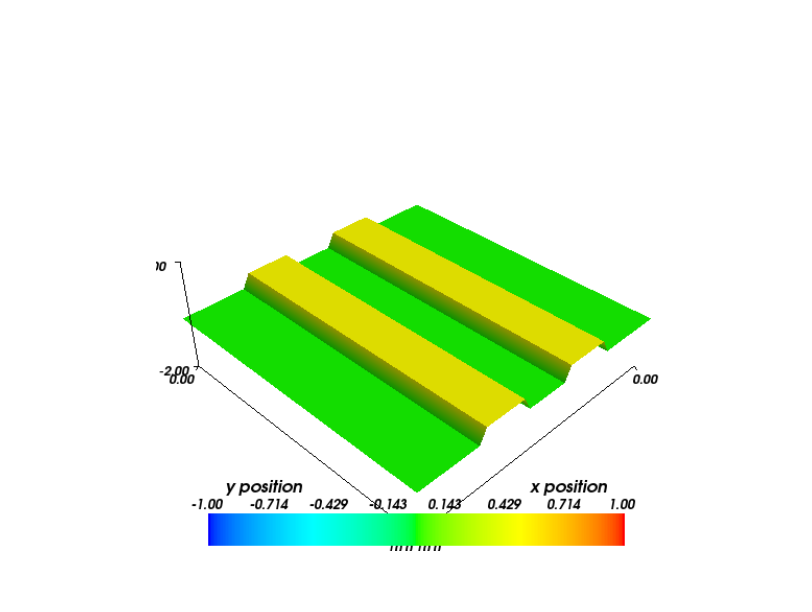
\includegraphics[width=13cm]{mayavitest.png}
\caption{The figure shows a screenshot of a stored animation of the plug wave solution}
\label{fig:mayavitest}
\end{figure}
\end{document}